\title{Mean Blur Filter Homework Assignment}
\author{
        Maruan Bakri Ottoni \\
        RA: 222025\\
        FEEC\\
        UNICAMP\\
        Campinas, \underline{Brazil}
}
\date{\today}
\documentclass[12pt]{article}
\usepackage[dvipsnames]{xcolor}
\usepackage{fancyvrb}
\usepackage{float}
\usepackage{graphicx}
\RecustomVerbatimCommand{\VerbatimInput}{VerbatimInput}%
{fontsize=\footnotesize,
 frame=lines,
 framesep=2em,
 rulecolor=\color{Gray},
 label=\fbox{\color{Black}data.txt},
 labelposition=topline,
 commandchars=\|\(\),
 commentchar=*
}

\begin{document}
\maketitle

\begin{abstract}
    Here on this homework assignment the mainline of work was to test three different approaches in trying to implement a median
    blur filter: Only one line of execution of the main program, Multithread and Multiprocess. I tested a hundred times each one of those
    alternatives and the result was that the user time of a multiprocess solution was in general, faster. In the case of real time the multithread and
    the multiprocess where equally good with a slight improve in performance in the multhread approach.
\end{abstarct}

\section{Images and the Final Result}
     \begin{figure}[H]
         \caption{Original image (Here will always appear the lena image. If you find necessary to change it, you have to modify the template.tex file).}
        \centering
        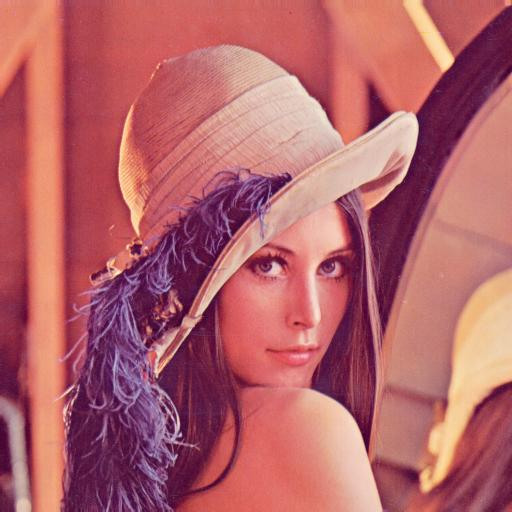
\includegraphics[width=8cm]{data/lena.jpg}
    \end{figure}
    \begin{figure}[H]
        \caption{Blur filter.}
        \centering
        
\includegraphics[width=8cm]{data/out.jpg}
    \end{figure}
\section{User time}
    \begin{figure}[H]
        \caption{User time graphic with only one line of execution.}
        \centering
        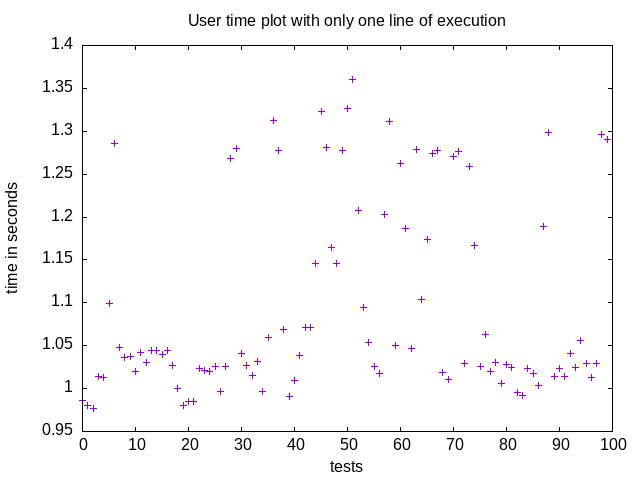
\includegraphics[width=8cm]{doc/user_simples.png}
    \end{figure}
    \VerbatimInput{doc/user_simples.log}

    \begin{figure}[H]
        \caption{User time graphic for a multiprocess approach.}
        \centering
        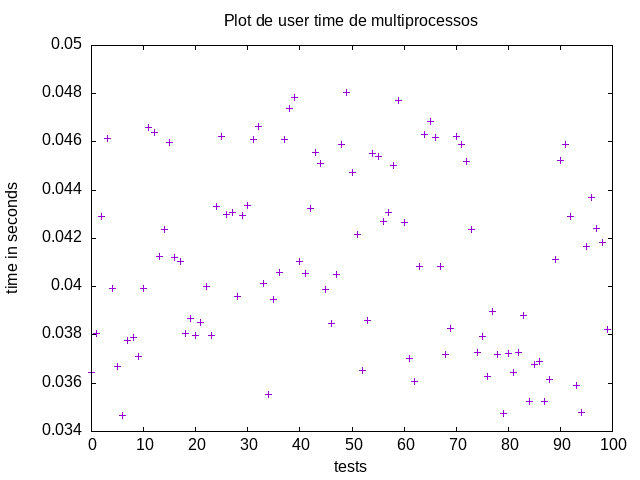
\includegraphics[width=8cm]{doc/user_processos.png}
    \end{figure}
    \VerbatimInput{doc/user_processos.log}

    \begin{figure}[H]
        \caption{User time graphic for a multithread approach.}
        \centering
        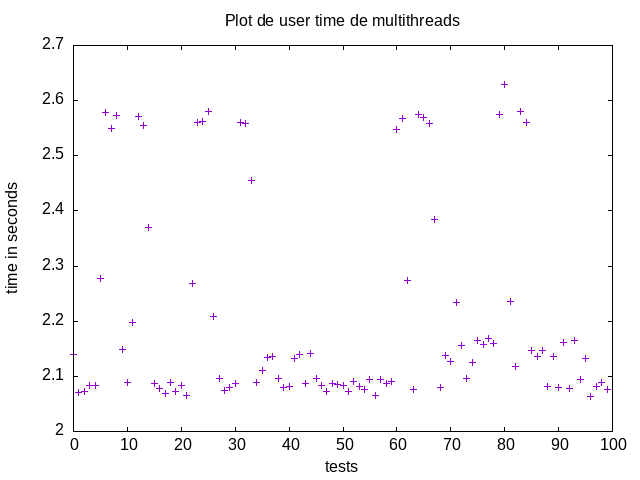
\includegraphics[width=8cm]{doc/user_threads.png}
    \end{figure}
    \VerbatimInput{doc/user_threads.log}


\section{Real Time}\label{results}
    \begin{figure}[H]
        \caption{Real time graphic for only one main line of execution.}
        \centering
        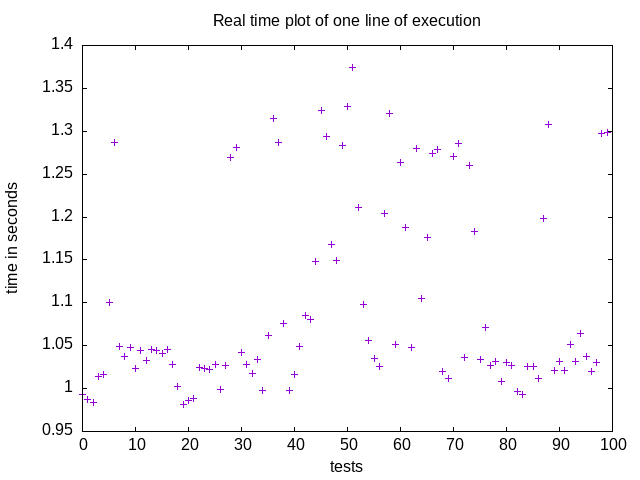
\includegraphics[width=8cm]{doc/real_simples.png}
    \end{figure}
    \VerbatimInput{doc/real_simples.log}

    \begin{figure}[H]
        \caption{Real Time grpahic for a multiprocess approach.}
        \centering
        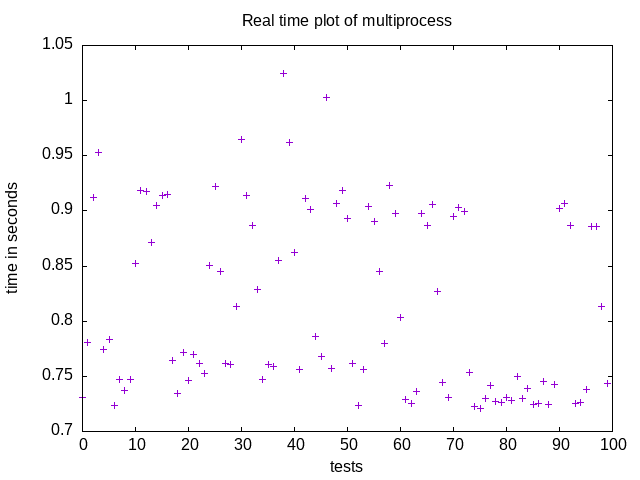
\includegraphics[width=8cm]{doc/real_processos.png}
    \end{figure}
    \VerbatimInput{doc/real_processos.log}

    \begin{figure}[H]
        \caption{Multithread real time graphic.}
        \centering
        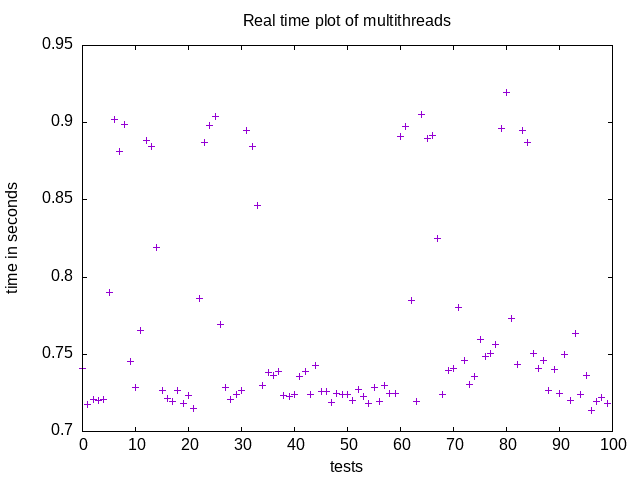
\includegraphics[width=8cm]{doc/real_threads.png}
    \end{figure}
    \VerbatimInput{doc/real_threads.log}

\section{Observation on the Real and User Time:}
\subsection{User Time}
User time is the amount of CPU time spent in user-mode code (outside the kernel) within the process. This is only actual CPU time used in executing the process. Other processes and time the process spends blocked do not count towards this figure.
\subsection{Real Time}
Real time is wall clock time - time from start to finish of the call. This is all elapsed time including time slices used by other processes and time the process spends blocked (for example ifit is waiting for I/O to complete).

\end{document}
